\section{Related Work}
%! 'As we do not propose any kind of new algorithm,' wouldn't it be better to just remove this? This sounds devaluing to the work.
%! '...and the actual classification...' is the word 'actual' necessary?
As we do not propose any kind of new algorithm, we will make use of existing solutions for both
the computation of the colour corrected image, and the actual classification of the images.

%! Good for report, but for the final paper replace 'we can make use of' with 'we used'.
To evaluate our results, we can make use of the publicly available Oxford 17 \cite{Nilsback06} 
and Oxford 104 \cite{Nilsback08} class datasets.

\subsection{Color Constancy}

\begin{figure}
    \centering
    \begin{tabular}{c|cccc}
    \bmvaHangBox{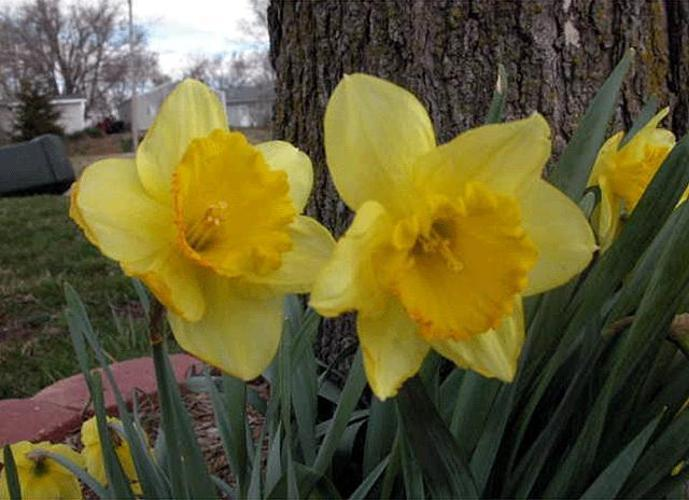
\includegraphics[width=0.165\textwidth]{cc_demo/flower001_base.png}}&
    \bmvaHangBox{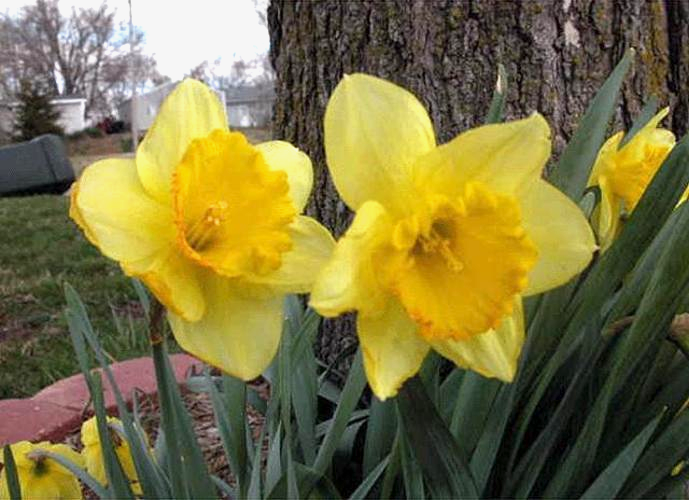
\includegraphics[width=0.165\textwidth]{cc_demo/flower001_whitePatch.png}}&
    \bmvaHangBox{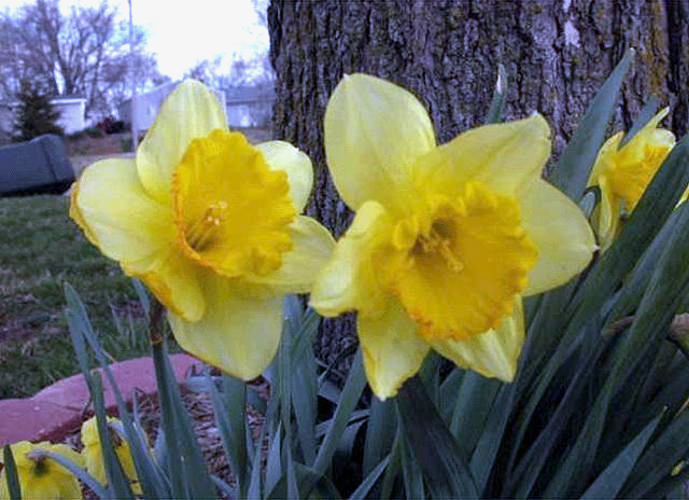
\includegraphics[width=0.165\textwidth]{cc_demo/flower001_greyWorld.png}}&
    \bmvaHangBox{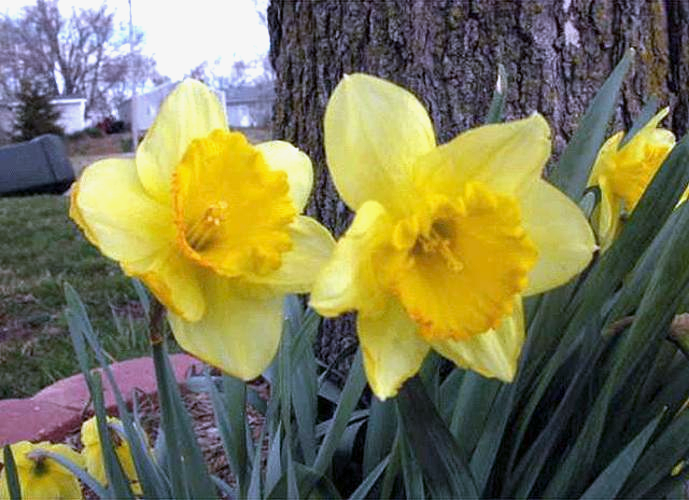
\includegraphics[width=0.165\textwidth]{cc_demo/flower001_grayEdge.png}}&
    \bmvaHangBox{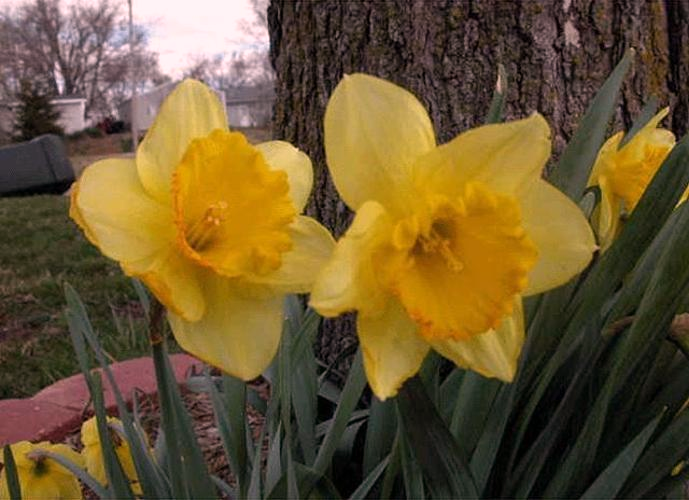
\includegraphics[width=0.165\textwidth]{cc_demo/flower001_fc4.png}}\\
    (a)&(b)&(c)&(d)&(e)\\
    \bmvaHangBox{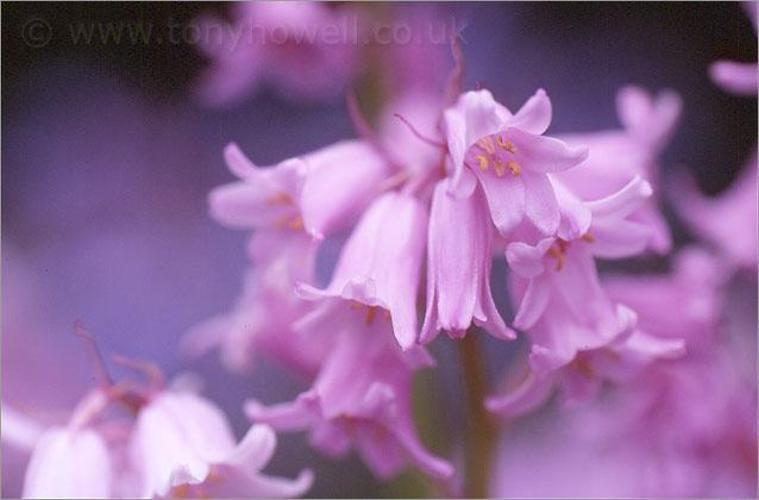
\includegraphics[width=0.165\textwidth]{cc_demo/flower268_base.png}}&
    \bmvaHangBox{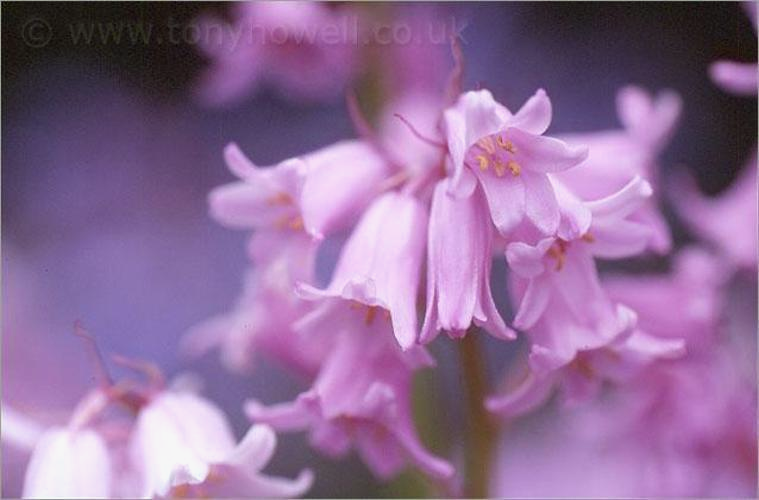
\includegraphics[width=0.165\textwidth]{cc_demo/flower268_whitePatch.png}}&
    \bmvaHangBox{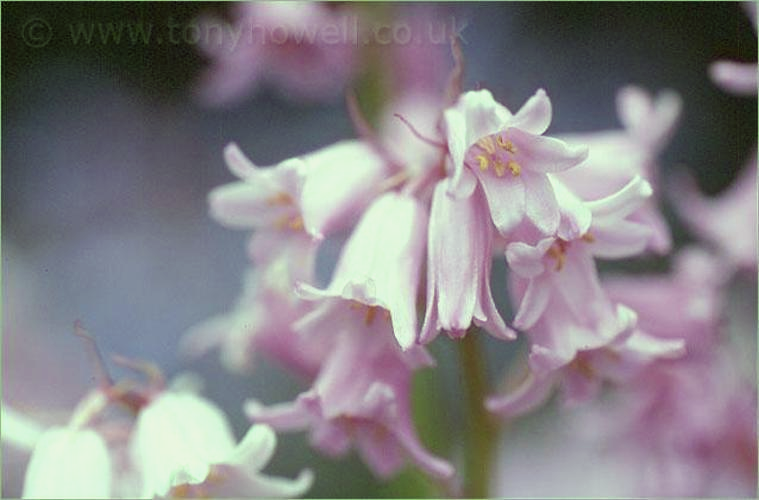
\includegraphics[width=0.165\textwidth]{cc_demo/flower268_greyWorld.png}}&
    \bmvaHangBox{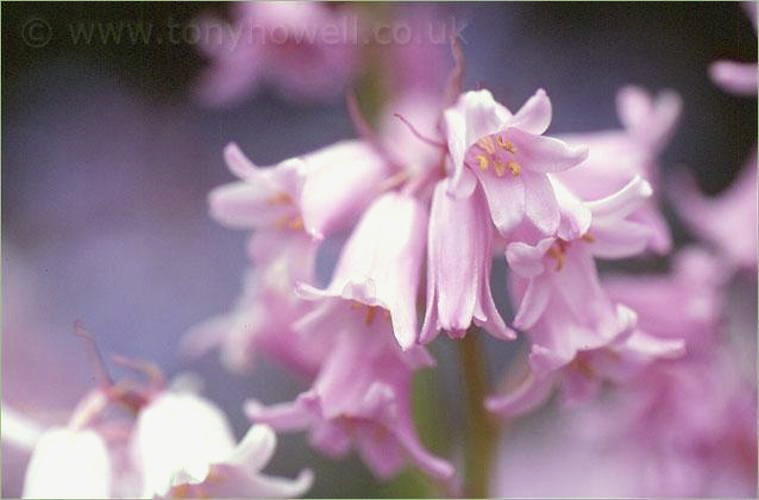
\includegraphics[width=0.165\textwidth]{cc_demo/flower268_grayEdge.png}}&
    \bmvaHangBox{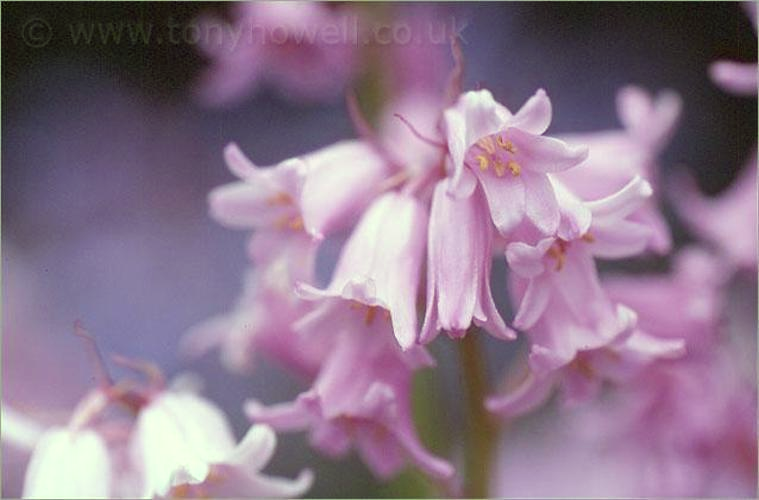
\includegraphics[width=0.165\textwidth]{cc_demo/flower268_fc4.png}}\\
    (f)&(g)&(h)&(i)&(j)
    \end{tabular}
    \caption{A comparison of color constancy algorithms: (a) and (f): Original image.
        (b) and (g): White Patch. (c) and (h): Grey-World. 
        (d) and (i): Grey-Edge. (e) and (j): FC\textsuperscript{4}}
    \label{fig:cc_comparison}
\end{figure}

In order to have a wider spread of examined methods, we both make use of state-of-the art 
learning based methods like CLCC \cite{Lo_2021_CVPR} and FC\textsuperscript{4}\cite{hu2017fc}, as well as classical simpler methods 
like White-Patch, Grey-World \cite{EbnerConstancy} and Grey-Edge \cite{van2005color}.
A comparison of these can be found in \ref{fig:cc_comparison}.

